\chapter{Introdução}
\label{cap1:introducao}
\pagestyle{plain}
\section{Contextualização}
O mercado tem se tornado cada vez mais competitivo, isso faz com que situações para diminuição dos custos de operação sejam adotadas, dentre tantas, pode-se citar o reuso de código, assim, técnicas para utilização desse meio são operacionalizadas, ainda mais com a inclusão de indicadores de retorno de investimento, um exemplo é o da \ref{fig:roi} que permitem realizar análise mais aprimorada a respeito do sucesso ou insucesso de um produto de software \cite{Weiss:1999:SPE:317887}. 

Com base nesse cenário, agilidade no desenvolvimento e qualidade de um produto tornam-se fatores decisivos. A reutilização de código e diminuição de etapas no processo de desenvolvimento de software são técnicas que veem sendo adotadas pela acadêmia e pela indústria ao longos dos anos \cite{delamaro2017introduccao}.

Abordagens veem sendo desenvolvidas com o propósito de aumentar a reusabilidade de software e, consequentemente, o retorno de investimento (ROI)  \cite{delamaro2017introduccao}. Entre essas abordagens está Linha de Produto de Software (LPS). LPS é uma alternativa de utilização como processo de desenvolvimento baseado em reuso de software, para se obter maior produtividade, reduzir custo, tempo e risco e proporcionar mais qualidade ao produto \cite{linden2007product}.

Uma LPS é um conjunto de sistemas de software que compartilham características (\textit{features}) comuns e gerenciáveis, que satisfazem as necessidades de um segmento particular ou de uma missão \cite{clements2002software}. Esse conjunto de sistemas é denominado também de família de produtos.

Uma LPS possui artefatos que podem ser reutilizados, assim, tendo em vista esse novo desafio de gerenciamento durante o desenvolvimento de software, os artefatos produzidos nos processos tradicionais de desenvolvimento de software já não são tão eficientes para o contexto de LPS, pois em sua maior parte não possuem suporte à variabilidade \cite{clements2002software}, em especial àquelas baseadas em UML. Assim, visando contornar esse problema, algumas abordagens têm sido propostas. 

Para o gerenciamento de variabilidade em LPS, \textit{Product Line UML-based Software Engineering} (PLUS) \cite{gomaa2006designing}, \cite{ziadi2003towards} e \textit{Stereotype-based Management of Variability} (\textit{SMarty}) \cite{junior2010systematic} são exemplos de tais abordagens. Essas abordagens usam estereótipos UML para representar variabilidade em elementos UML de uma LPS. Assim, dada uma LPS, um de seus maiores desafios é o seu teste, especialmente baseado em modelos que contém variabilidade, pois se torna inviável testar todos os possíveis produtos de uma LPS.

\section{Motivação e Justificativa}
\label{cap1sec:motivacao}

Embora teste de software ser amplamente difundido, assim como os conceitos de LPS, sua utilização de forma errônea, sem o conhecimento prévio ou de forma equivocada, sempre proporcionam pontos em que surgem dúvidas e onde deve-se tomar atenção com relação ao resultado final do desenvolvimento. Isso impacta diretamente na qualidade e custo de um produto de software, principalmente se tratando de uma LPS \cite{Weiss:1999:SPE:317887}. 

Na \ref{fig:roi} é apresentada uma comparação entre um cenário de desenvolvimento de sistema único e o de linha de produto. \citet{Weiss:1999:SPE:317887} afirmam com base em estudos que, o custo no desenvolvimento de sistemas únicos se eleva quando se aumenta a quantidade de produtos diferentes.


\begin{figure}[h]
	\centering
	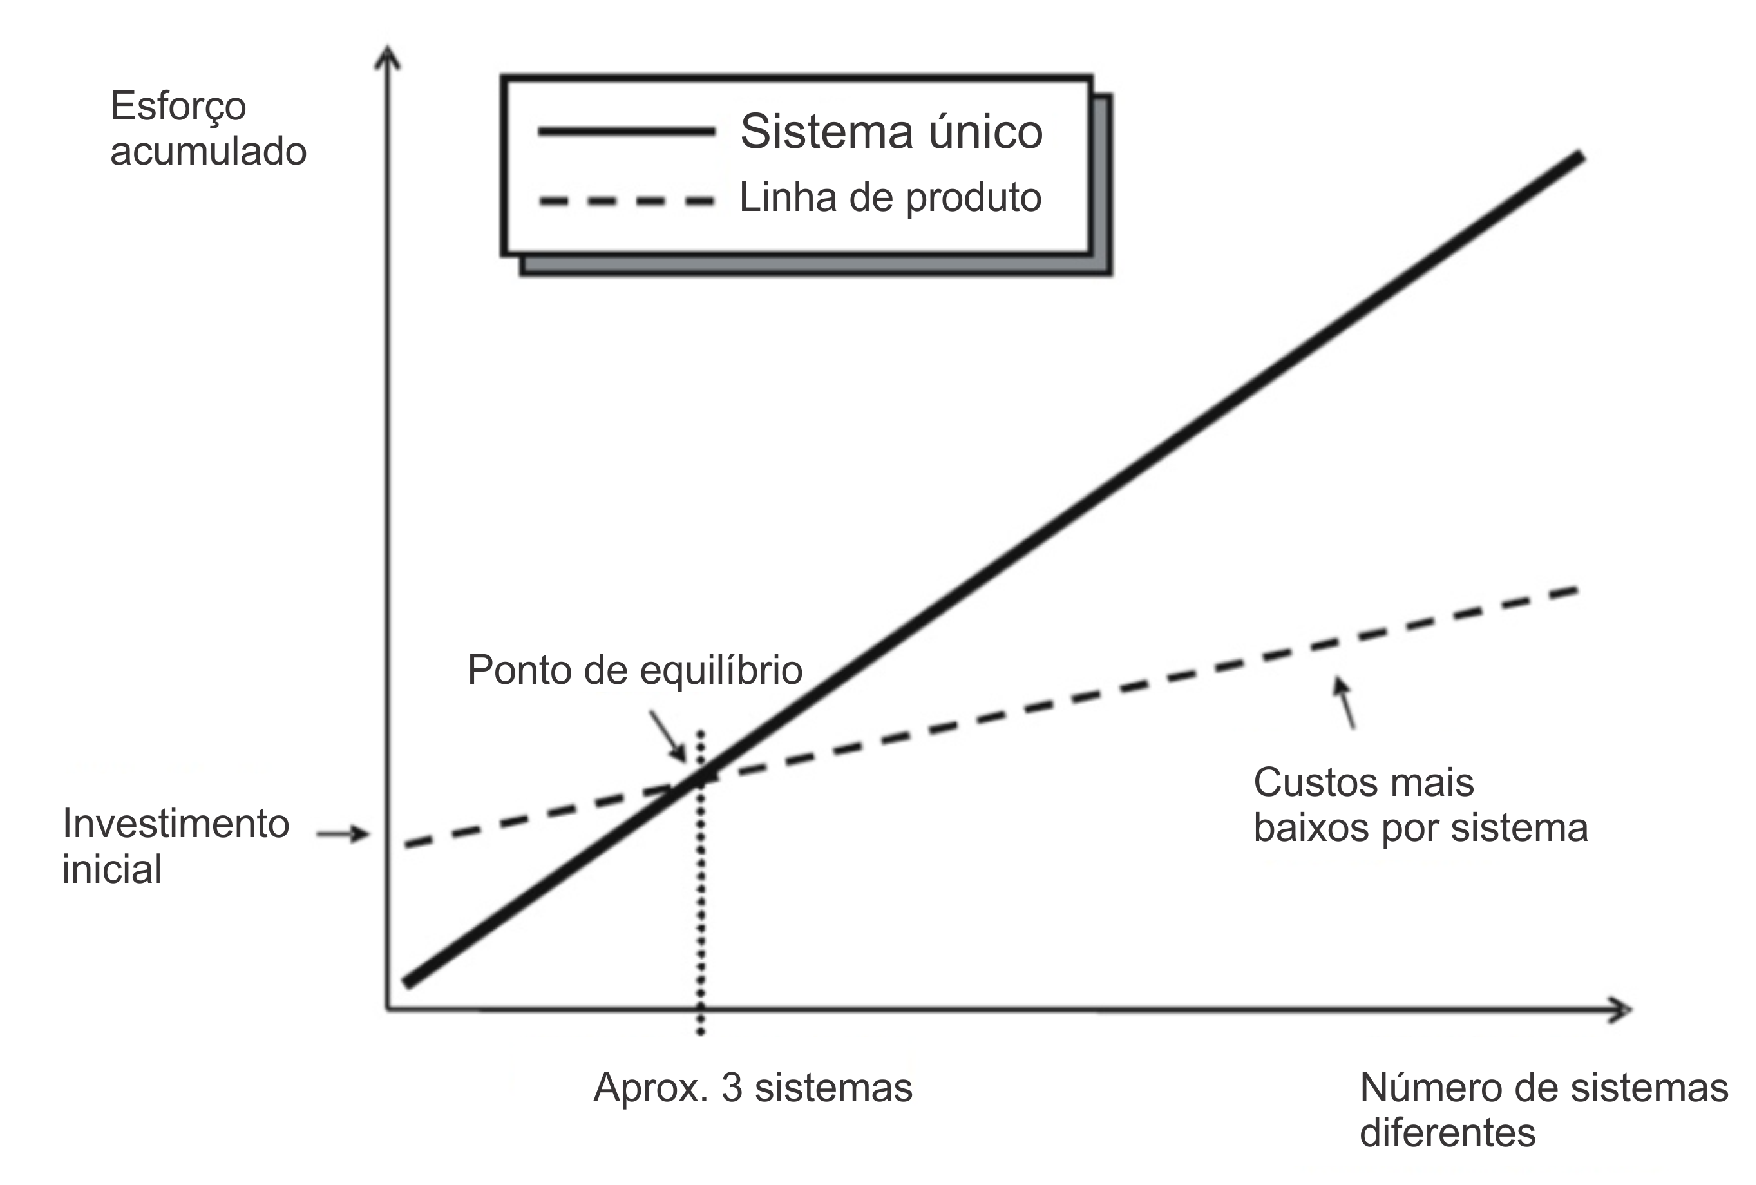
\includegraphics[scale=0.35]{roi_traduzido.pdf}
	\caption{Comparação entre desenvolvimento de sistemas únicos e linha de produtos \cite{Weiss:1999:SPE:317887}.}
	\label{fig:roi}
\end{figure}


Além do processo de execução e desafios da operação de teste em uma LPS, deve-se considerar as particularidades individuais de cada produto gerado e assim, tem-se um ponto que demanda atenção especial, que é a variabilidade \cite{engstrom2011software}. Testar uma LPS levando em consideração uma ampla cadeia de variações de produtos é um grande desafio, impactando diretamente nas métricas de qualidade seja quais que foram definidas \cite{junior2013systematic}. 

Existe um desafio muito grande na realização de testes para produtos derivados de LPS, pela quantidade de produtos semelhantes, e por suas particularidades que os diferem uns dos outros. Sobre esse ponto, considera-se neste trabalho que a variabilidade é gerenciada utilizando-se a abordagem \textit{SMarty} \cite{junior2010systematic}, visto que possui um perfil que permite que inspeções baseadas em \textit{checklist} sejam realizadas e que já foi amplamente avaliado. Isso motivou, a criação de um perfil voltado para a geração de sequências de testes baseados em modelos \textit{SMarty}, contribuindo, assim, para a antecipação dos casos de teste no ciclo de vida de LPS.

Outro motivo que norteia este trabalho é a suposição de que diagramas de sequência (DS) possam produzir mais sequências de teste que diagramas de atividades (DA).  Nesse caso, uma sequência pode conter mais casos de testes que várias sequências com poucos casos de teste. Dessa forma, a questão de pesquisa deste trabalho é \textbf{``Diagramas de sequência podem gerar mais sequências de teste do que diagramas de atividades?"} 

\section{Objetivo}
\label{cap1sec:objetivo}

Conforme a motivação apresentada, esta dissertação tem como objetivo principal especificar e viabilizar o desenvolvimento da abordagem \textit{SMartyTesting} para teste baseado em modelos \textit{SMarty} para LPS, considerando como modelo de partida diagramas de casos de uso e diagramas de sequência pelo alto grau de detalhes, informações, pelos quais pode ser representado. 


Assim, tem-se como objetivos específicos:
\begin{itemize}
	\item investigar na literatura, soluções que utilizam diagramas de sequência para o teste baseado em modelo de LPS;
	\item identificar uma forma de utilização de diagramas de sequência para a geração de sequências de testes que possam ser utilizados na criação de casos de teste; e
	\item analisar a viabilidade da abordagem proposta, com base em resultados de uma comparação entre diagramas de sequência e diagramas de atividades.
\end{itemize} 


\section{Metodologia de Desenvolvimento}
\label{cap1sec:metodo_desenv}


Para atingir o objetivo proposto neste trabalho foi necessário realizar as etapas apresentadas na \ref{fig:fluxometodo} como descrito a seguir:

\begin{figure}[h!]
	\centering
	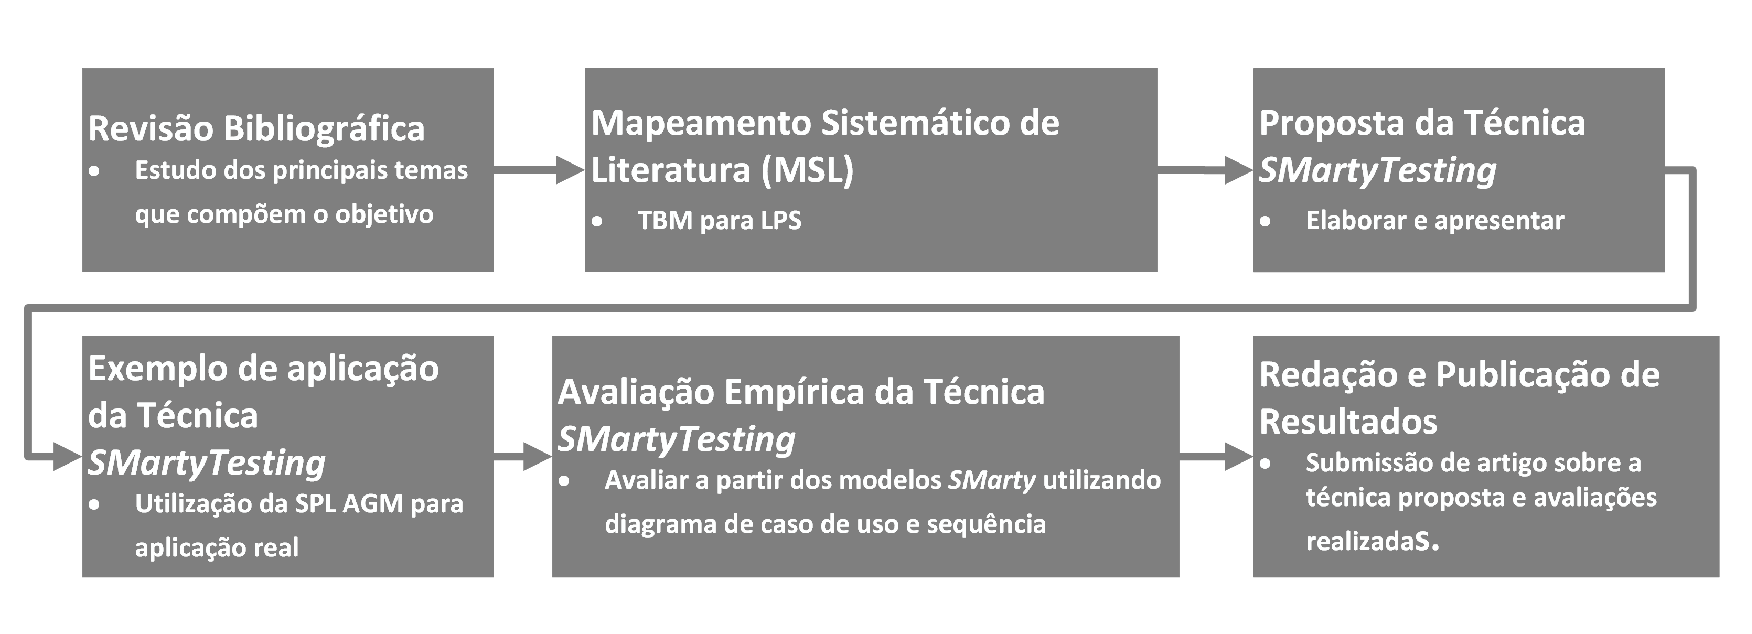
\includegraphics[scale=0.40]{fluxo_metodologia.pdf}
	\caption{Etapas da Metodologia de Desenvolvimento de Pesquisa}
	\label{fig:fluxometodo}
\end{figure}

\begin{itemize}
	\item \textbf{Revisão Bibliográfica:} foram estudados os conceitos sobre os principais temas que fazem parte do objetivo da pesquisa, tais como: perfis UML, diagramas de sequência, teste de LPS, conceitos de LPS, gerenciamento de variabilidade, a abordagem \textit{SMarty} e a abordagem SPLiT-MBt;
	
	\item \textbf{Estudo secundário:} foi realizado um Mapeamento Sistemático de Literatura (MSL), em que o tema abordado foi TBM para LPS. Tal estudo encontra-se no Apêndice \ref{sec:secmsl_MSL}. A análise dos estudos do MSL permitiu a identificação de formas diferenciadas de aplicação de TBM em LPS e permitiu embasar este trabalho;
	
	\item \textbf{Proposta da Abordagem \textit{SMartyTesting}:} foi definido um fluxo de trabalho para concepção e construção da abordagem, cujas etapas que a antecedem foram o embasamento teórico e a realização do mapeamento sistemático. Inicialmente foi realizado um trabalho de Mapeamento Sistemático de Literatura para embasamento da abordagem, após a análise dos dados, foi realizada a concepção da abordagem com os passos necessários para se alcançar o objetivo principal. Na fase de concepção, uma pesquisa sobre ferramentas de apoio foi desenvolvida e, em seguida, as mesmas foram validadas, para se saber qual delas poderia ser utilizada na abordagem \textit{SMartyTesting}. Por fim, foi realizado um estudo de viabilidade comparativo com SPLiT-MBt para a validação, e a proposta final foi concluída;
		
	\begin{figure}[h!]
		\centering
		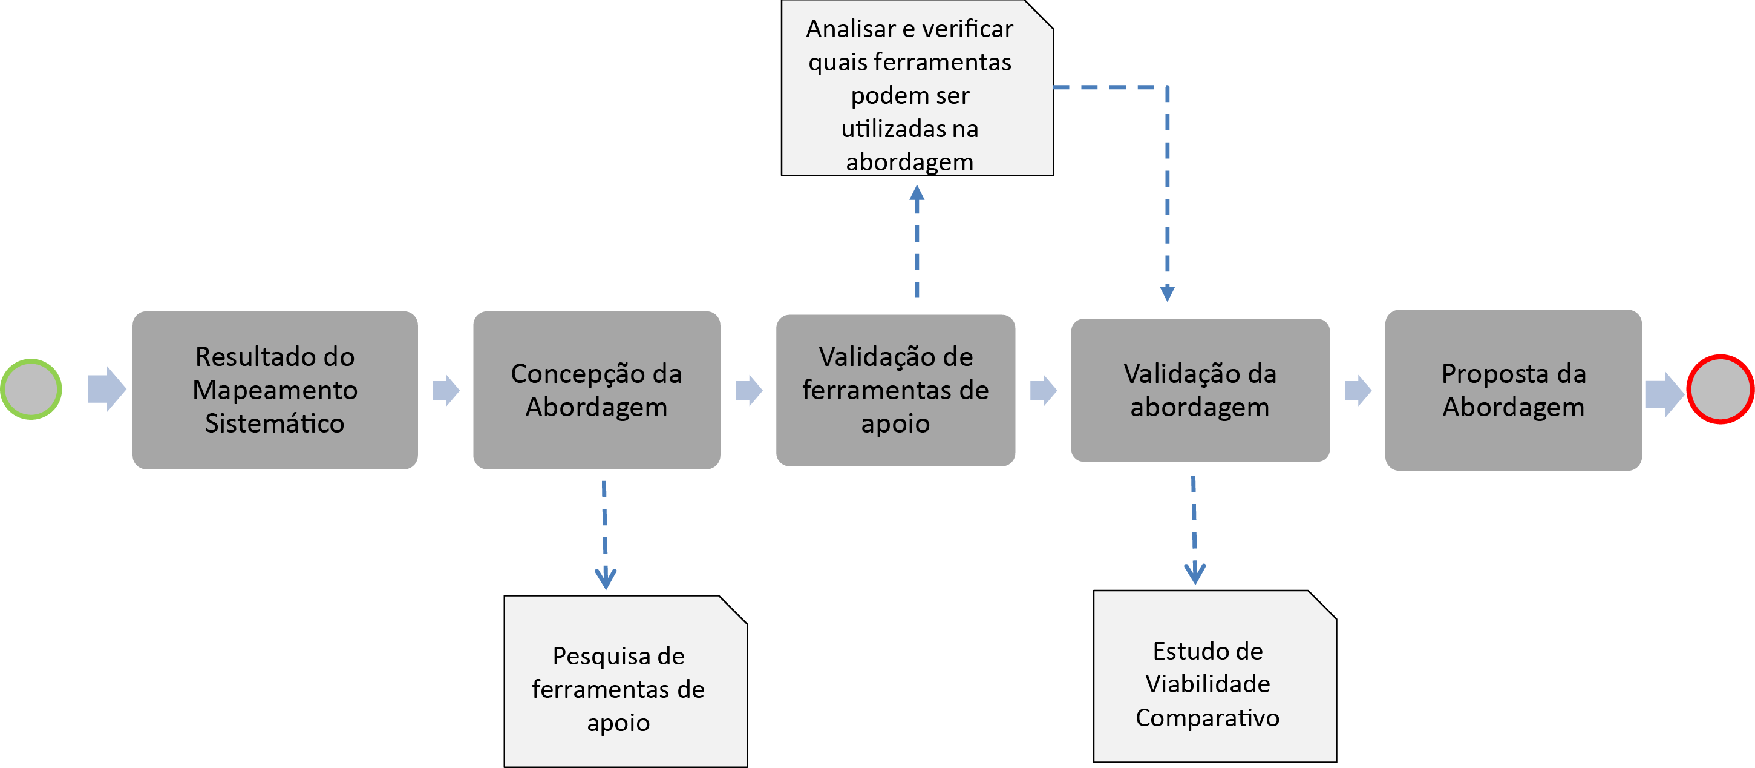
\includegraphics[scale=0.50]{ciclo_pesquisa2.pdf}
		\caption{Desenvolvimento da Abordagem \textit{SMartyTesting}}
		\label{fig:fluxopesquisa2}
	\end{figure}
	
	\item \textbf{Estudo de Viabilidade de \textit{SMartyTesting}:} foi realizado um estudo de viabilidade, considerando a abordagem \textit{SMartyTesting}, utilizando diagramas de sequência, com a abordagem SPLiT-MBt que utilizou diagramas de atividades. Com relação aos critérios de análise foram definidos quatro critérios que estão detalhados na Seção \ref{cap4subsec:criterios}; e
	
	\item \textbf{Melhorias e Lições Aprendidas:} as melhorias identificadas relacionadas às abordagens \textit{SMartyTesting} e SPLiT-MBt são discutidas com base nos resultados do estudo de viabilidade bem como as lições aprendidas com este trabalho (Tópico \ref{cap5:melhorias}).
\end{itemize}


\section{Organização do Texto}
\label{cap1sec:organizacao}
O trabalho está organizado como segue. No tópico 2 é apresentada a fundamentação teórica sobre LPS e a abordagem \textit{SMarty}, teste de LPS, Teste Baseado em Modelo (TBM) de LPS e a abordagem SPLiT-MBt que é uma das bases para este trabalho e diagramas de sequência e de atividades. No tópico 3 é descrita a abordagem proposta, assim como processos, modelos, ferramentas e meios para a aplicação e utilização de \textit{SMartyTesting}. O tópico 4 apresenta o estudo de viabilidade realizado. No tópico 5 são discutidas as melhorias identificadas e lições aprendidas para as abordagens \textit{SMartyTesting} e SPLiT-MBt. O tópico 6  apresenta conclusões, limitações e trabalhos futuros desta dissertação. 


